\documentclass{article}
\usepackage{tikz}
\usetikzlibrary{intersections}
\usetikzlibrary{snakes}
\usetikzlibrary{decorations}
\usetikzlibrary{decorations.text}
\usetikzlibrary{shapes}
\usetikzlibrary{arrows}
\usetikzlibrary{automata}
\usetikzlibrary{positioning}
\usetikzlibrary{shadows}
\usetikzlibrary{matrix}
\usetikzlibrary{patterns}
\usepgfmodule{plot}

\title{Silviu's TikZ Test Cases}
\begin{document}
%======================================================================
\section{Environments}
\begingroup % ------ pseudo document ---------
Rectangles
\begin{pgfpicture}
  \pgfpathrectangle{\pgfpointorigin}{\pgfpoint{2ex}{1ex}}
  \pgfusepath{stroke}
\end{pgfpicture}
 and
\begin{pgfpicture}
  \pgfpathrectangle{\pgfpoint{0ex}{1ex}}{\pgfpoint{2ex}{1ex}}
  \pgfusepath{stroke}
\end{pgfpicture}.
Inline
\tikz{\pgfpathcircle{\pgfpointorigin}{1ex}\pgfusepath{stroke}}.
Hello
%\tikz{
%\pgfsetbaselinepointlater{\pgfpointanchor{X}{base}}
% Note: no shape X, yet
%\node [cross out,draw] (X) {world.};
%}
\endgroup % ----------- end -----------------
%======================================================================
\section{Scopes}
\begingroup % ------ pseudo document ---------
\begin{pgfpicture}
  \begin{pgfscope}
  {
  \pgfsetlinewidth{2pt}
  \pgfpathrectangle{\pgfpointorigin}{\pgfpoint{2ex}{2ex}}
  \pgfusepath{stroke}
  }
  \pgfpathrectangle{\pgfpoint{3ex}{0ex}}{\pgfpoint{2ex}{2ex}}
  \pgfusepath{stroke}
  \end{pgfscope}
  \pgfpathrectangle{\pgfpoint{6ex}{0ex}}{\pgfpoint{2ex}{2ex}}
  \pgfusepath{stroke}
\end{pgfpicture}
\endgroup % ----------- end -----------------
%======================================================================
\section{Coordinates}
\begingroup % ------ pseudo document ---------
% TODO: Need to deal with color scoping
% TODO: Relevantforpicturesize: should I manually increase a bit by half the size of the text?
%
% Basic coordinate commands
%
Points

% Testing \pgfpoint
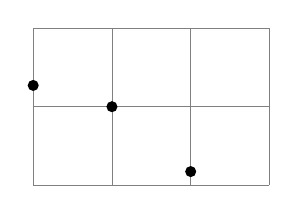
\begin{tikzpicture}
  \draw[help lines] (0,0) grid (3,2);
  \pgfpathcircle{\pgfpoint{1cm}{1cm}} {2pt}
  \pgfpathcircle{\pgfpoint{2cm}{5pt}} {2pt}
  \pgfpathcircle{\pgfpoint{0pt}{.5in}}{2pt}
  \pgfusepath{fill}
\end{tikzpicture}
% Testing \pgfpointpolar
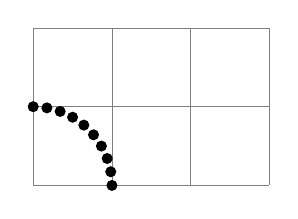
\begin{tikzpicture}
  \draw[help lines] (0,0) grid (3,2);
  \foreach \angle in {0,10,...,90}{
     \pgfpathcircle{\pgfpointpolar{\angle}{1cm}}{2pt}}
   \pgfusepath{fill}
\end{tikzpicture}
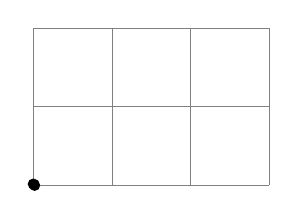
\begin{tikzpicture}
  \draw[help lines] (0,0) grid (3,2);
  \foreach \angle in {0,10,...,90}{
    \pgfpathcircle{\pgfpointpolar{\angle}{1cm/2cm}}{2pt}}
  \pgfusepath{fill}
\end{tikzpicture}
%

2d coordinates

% Testing \pgfpointxy
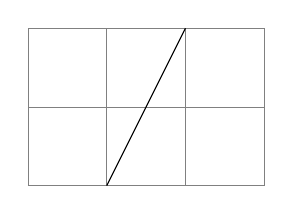
\begin{tikzpicture}
  \draw[help lines] (0,0) grid (3,2);
  \pgfpathmoveto{\pgfpointxy{1}{0}}
  \pgfpathlineto{\pgfpointxy{2}{2}}
  \pgfusepath{stroke}
\end{tikzpicture}
% Testing \pgfset(x|y)vec
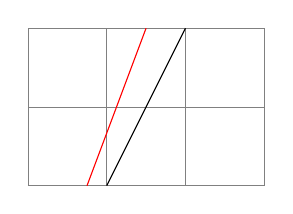
\begin{tikzpicture}
  \draw[help lines] (0,0) grid (3,2);
  \pgfpathmoveto{\pgfpointxy{1}{0}}
  \pgfpathlineto{\pgfpointxy{2}{2}}
  \pgfusepath{stroke}
  \color{red}
  \pgfsetxvec{\pgfpoint{0.75cm}{0cm}}
  \pgfpathmoveto{\pgfpointxy{1}{0}}
  \pgfpathlineto{\pgfpointxy{2}{2}}
  \pgfusepath{stroke}
\end{tikzpicture}
% Testing \pgfpointpolarxy
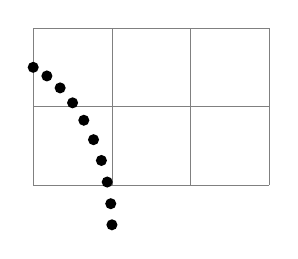
\begin{tikzpicture}
  \draw[help lines] (0,0) grid (3,2);
  \begin{scope}[x={(1cm,-5mm)},y=1.5cm]
    \foreach \angle in {0,10,...,90}{
       \pgfpathcircle{\pgfpointpolarxy{\angle}{1}}{2pt}}
    \pgfusepath{fill}
  \end{scope}
\end{tikzpicture}

3d coordinates

% Testing \pgfpointxyz
\begin{pgfpicture}
  \pgfsetarrowsend{to}
  \pgfpathmoveto{\pgfpointorigin}
  \pgfpathlineto{\pgfpointxyz{0}{0}{1}}
  \pgfusepath{stroke}
  \pgfpathmoveto{\pgfpointorigin}
  \pgfpathlineto{\pgfpointxyz{0}{1}{0}}
  \pgfusepath{stroke}
  \pgfpathmoveto{\pgfpointorigin}
  \pgfpathlineto{\pgfpointxyz{1}{0}{0}}
  \pgfusepath{stroke}
\end{pgfpicture}
% Testing \pgfpointcylindrical
\begin{tikzpicture}
  \draw [->] (0,0) -- (1,0,0) node [right] {x};
  \draw [->] (0,0) -- (0,1,0) node [above] {y};
  \draw [->] (0,0) -- (0,0,1) node [below left] {z};
  \pgfpathcircle{\pgfpointcylindrical{80}{1}{.5}}{2pt}
  \pgfusepath{fill}
  \draw[red] (0,0) -- (0,0,.5) -- +(80:1);
\end{tikzpicture}
% Testing \pgfpointspherical
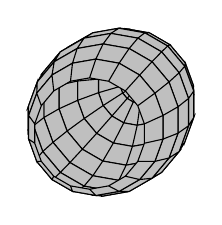
\begin{tikzpicture}
  \pgfsetfillcolor{lightgray}
  \foreach \latitude in {-90,-75,...,30}{
    \foreach \longitude in {0,20,...,360}{
       \pgfpathmoveto{\pgfpointspherical{\longitude}{\latitude}{1}}
       \pgfpathlineto{\pgfpointspherical{\longitude+20}{\latitude}{1}}
       \pgfpathlineto{\pgfpointspherical{\longitude+20}{\latitude+15}{1}}
       \pgfpathlineto{\pgfpointspherical{\longitude}{\latitude+15}{1}}
       \pgfpathclose
     }
     \pgfusepath{fill,stroke}
   }
\end{tikzpicture}
\endgroup % ----------- end -----------------

\begingroup % ------ pseudo document ---------
Basic manipulation of coordinates

% Testing \pgfpointadd
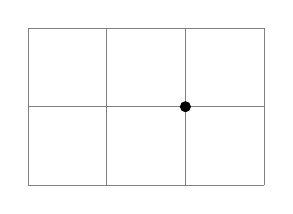
\begin{tikzpicture}
  \draw[help lines] (0,0) grid (3,2);
  \pgfpathcircle{\pgfpointadd{\pgfpoint{1cm}{0cm}}{\pgfpoint{1cm}{1cm}}}{2pt}
  \pgfusepath{fill}
\end{tikzpicture}
% Testing \pgfpointscale
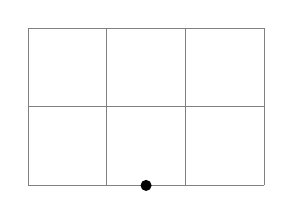
\begin{tikzpicture}
  \draw[help lines] (0,0) grid (3,2);
  \pgfpathcircle{\pgfpointscale{1.5}{\pgfpoint{1cm}{0cm}}}{2pt}
  \pgfusepath{fill}
\end{tikzpicture}
% Testing \pgfpointdiff
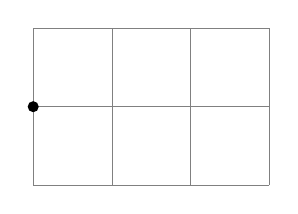
\begin{tikzpicture}
  \draw[help lines] (0,0) grid (3,2);
  \pgfpathcircle{\pgfpointdiff{\pgfpoint{1cm}{0cm}}{\pgfpoint{1cm}{1cm}}}{2pt}
  \pgfusepath{fill}
\end{tikzpicture}
% Testing \pgfointnormalised
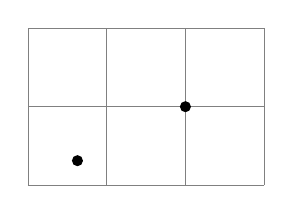
\begin{tikzpicture}
  \draw[help lines] (0,0) grid (3,2);
  \pgfpathcircle{\pgfpoint{2cm}{1cm}}{2pt}
  \pgfpathcircle{\pgfpointscale{20}{\pgfpointnormalised{\pgfpoint{2cm}{1cm}}}}{2pt}
\pgfusepath{fill}
\end{tikzpicture}

Points along lines and curves

% Testing \pgfpointlineattime
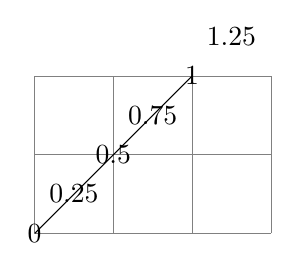
\begin{tikzpicture}
  \draw[help lines] (0,0) grid (3,2);
  \pgfpathmoveto{\pgfpointorigin}
  \pgfpathlineto{\pgfpoint{2cm}{2cm}}
  \pgfusepath{stroke}
  \foreach \t in {0,0.25,...,1.25}{
    \pgftext[at=\pgfpointlineattime{\t}{\pgfpointorigin}{\pgfpoint{2cm}{2cm}}]{\t}}
\end{tikzpicture}
% \pgfpointlineatdistance
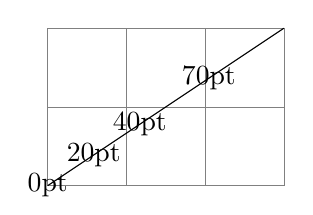
\begin{tikzpicture}
  \draw[help lines] (0,0) grid (3,2);
  \pgfpathmoveto{\pgfpointorigin}
  \pgfpathlineto{\pgfpoint{3cm}{2cm}}
  \pgfusepath{stroke}
  \foreach \d in {0pt,20pt,40pt,70pt}{
    \pgftext[at=\pgfpointlineatdistance{\d}{\pgfpointorigin}{\pgfpoint{3cm}{2cm}}]{\d}}
\end{tikzpicture}
% \pgfpointcurveattime
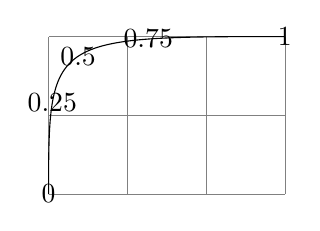
\begin{tikzpicture}
  \draw[help lines] (0,0) grid (3,2);
  \pgfpathmoveto{\pgfpointorigin}
  \pgfpathcurveto{\pgfpoint{0cm}{2cm}}{\pgfpoint{0cm}{2cm}}{\pgfpoint{3cm}{2cm}}
  \pgfusepath{stroke}
  \foreach \t in {0,0.25,0.5,0.75,1}{
    \pgftext[at=\pgfpointcurveattime{\t}{
      \pgfpointorigin}{\pgfpoint{0cm}{2cm}}{\pgfpoint{0cm}{2cm}}{\pgfpoint{3cm}{2cm}}]{\t}}
\end{tikzpicture}

Points on borders of objects

% \pgfpointborderrectangle
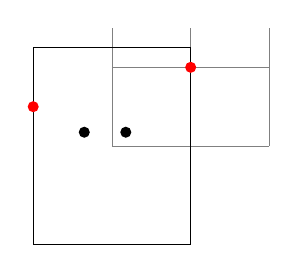
\begin{tikzpicture}
  \draw[help lines] (0,0) grid (2,1.5);
  \pgfpathrectanglecorners{\pgfpoint{-1cm}{-1.25cm}}{\pgfpoint{1cm}{1.25cm}}
  \pgfusepath{stroke}
  \pgfpathcircle{\pgfpoint{5pt}{5pt}}{2pt}
  \pgfpathcircle{\pgfpoint{-10pt}{5pt}}{2pt}
  \pgfusepath{fill}
  \color{red}
  \pgfpathcircle{\pgfpointborderrectangle{\pgfpoint{5pt}{5pt}}{\pgfpoint{1cm}{1.25cm}}}{2pt}
  \pgfpathcircle{\pgfpointborderrectangle{\pgfpoint{-10pt}{5pt}}{\pgfpoint{1cm}{1.25cm}}}{2pt}
  \pgfusepath{fill}
\end{tikzpicture}
% \pgfborderellipse
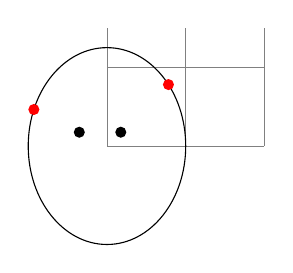
\begin{tikzpicture}
  \draw[help lines] (0,0) grid (2,1.5);
  \pgfpathellipse{\pgfpointorigin}{\pgfpoint{1cm}{0cm}}{\pgfpoint{0cm}{1.25cm}}
  \pgfusepath{stroke}
  \pgfpathcircle{\pgfpoint{5pt}{5pt}}{2pt}
  \pgfpathcircle{\pgfpoint{-10pt}{5pt}}{2pt}
  \pgfusepath{fill}
  \color{red}
  \pgfpathcircle{\pgfpointborderellipse{\pgfpoint{5pt}{5pt}}{\pgfpoint{1cm}{1.25cm}}}{2pt}
  \pgfpathcircle{\pgfpointborderellipse{\pgfpoint{-10pt}{5pt}}{\pgfpoint{1cm}{1.25cm}}}{2pt}
  \pgfusepath{fill}
\end{tikzpicture}

Points on intersections of lines

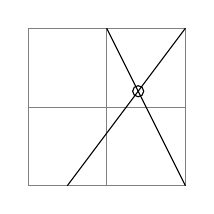
\begin{tikzpicture}
  \draw[help lines] (0,0) grid (2,2);
  \draw (.5,0) -- (2,2);
  \draw (1,2) -- (2,0);
  \pgfpathcircle{%
   \pgfpointintersectionoflines{\pgfpointxy{.5}{0}}{\pgfpointxy{2}{2}}
    {\pgfpointxy{1}{2}}{\pgfpointxy{2}{0}}}{2pt}
\pgfusepath{stroke}
\end{tikzpicture}
%
% Points on intersections of circles
%
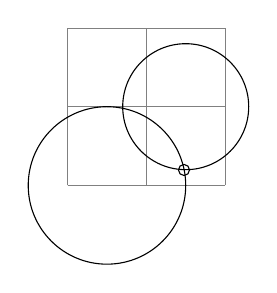
\begin{tikzpicture}
  \draw[help lines] (0,0) grid (2,2);
  \draw (0.5,0) circle (1);
  \draw (1.5,1) circle (.8);
  \pgfpathcircle{%
  \pgfpointintersectionofcircles{\pgfpointxy{.5}{0}}{\pgfpointxy{1.5}{1}}{1cm}{0.8cm}{1}}{2pt}
  \pgfusepath{stroke}
\end{tikzpicture}
%
% Points on intersections of paths
%
\begin{pgfpicture}
  \pgfintersectionofpaths{
    \pgfpathellipse{\pgfpointxy{0}{0}}{\pgfpointxy{1}{0}}{\pgfpointxy{0}{2}}
    \pgfgetpath\temppath
    \pgfusepath{stroke}
    \pgfsetpath\temppath
   }
   {
     \pgftransformrotate{-30}
     \pgfpathrectangle{\pgfpointorigin}{\pgfpointxy{2}{2}}
     \pgfgetpath\temppath
     \pgfusepath{stroke}
     \pgfsetpath\temppath
   }
   \foreach \s in {1,...,\pgfintersectionsolutions}{
      \pgfpathcircle{\pgfpointintersectionsolution{\s}}{2pt}}
   \pgfusepath{stroke}
\end{pgfpicture}
\endgroup % ----------- end -----------------
%======================================================================
\section{Paths}

\begingroup % ------ pseudo document ---------
% General cooler test
General:
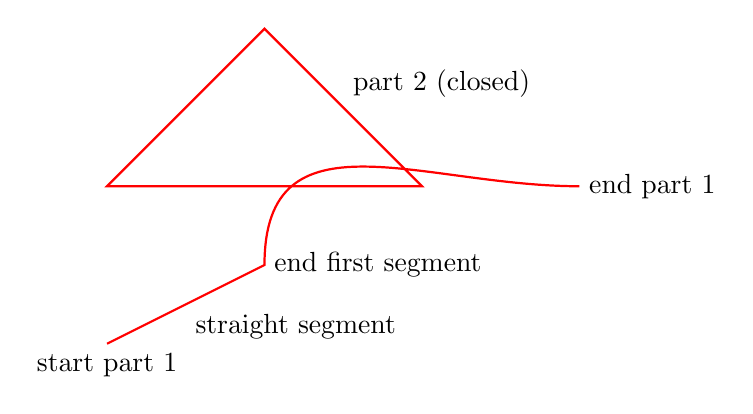
\begin{tikzpicture}[scale=2]
  \draw[thick,red]
    (0,0) coordinate (a)
    -- coordinate (ab)
    (1,.5) coordinate (b)
    .. coordinate (bc)
    controls +(up:1cm) and +(left:1cm)
    .. (3,1) coordinate (c)
    (0,1) -- (2,1)
    -- coordinate (x) (1,2)
    -- cycle;
  \draw (a) node[below] {start part 1}
    (ab) node[below right] {straight segment}
    (b) node[right] {end first segment}
    (c) node[right] {end part 1}
    (x) node[above right] {part 2 (closed)};
\end{tikzpicture}

pgfpath(moveto,lineto,curveto):
\begin{pgfpicture}[scale=2]
  \pgfpathmoveto{\pgfpointorigin}
  \pgfpathlineto{\pgfpoint{1cm}{1cm}}
  \pgfpathlineto{\pgfpoint{2cm}{1cm}}
  \pgfpathcurveto{\pgfpoint{1cm}{1cm}}{\pgfpoint{4cm}{1cm}}{\pgfpoint{3cm}{0cm}}
  \pgfsetfillcolor{yellow}
  \pgfusepath{fill,stroke}
\end{pgfpicture}

pgfclosepath:
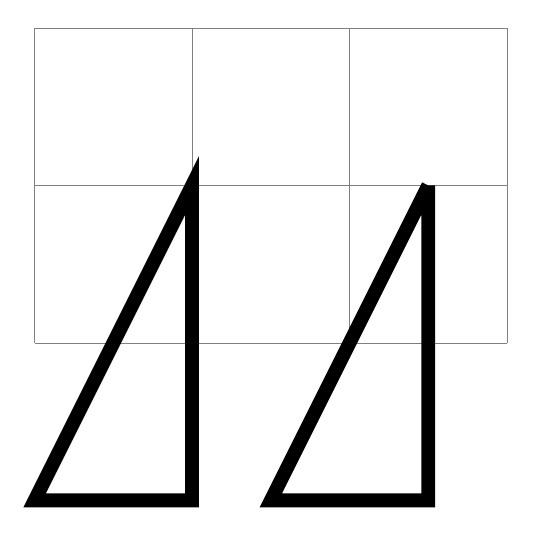
\begin{tikzpicture}[scale=2]
  \draw[help lines] (0,0) grid (3,2);
  \pgfsetlinewidth{5pt}
  \pgfpathmoveto{\pgfpoint{1cm}{1cm}}
  \pgfpathlineto{\pgfpoint{0cm}{-1cm}}
  \pgfpathlineto{\pgfpoint{1cm}{-1cm}}
  \pgfpathclose
  \pgfpathmoveto{\pgfpoint{2.5cm}{1cm}}
  \pgfpathlineto{\pgfpoint{1.5cm}{-1cm}}
  \pgfpathlineto{\pgfpoint{2.5cm}{-1cm}}
  \pgfpathlineto{\pgfpoint{2.5cm}{1cm}}
  \pgfusepath{stroke}
\end{tikzpicture}

pgfpath(arc,arcaxes):
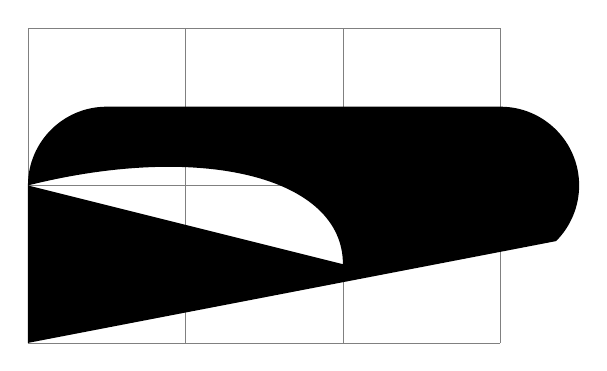
\begin{tikzpicture}[scale=2]
  \draw[help lines] (0,0) grid (3,2);
  \pgfpathmoveto{\pgfpointorigin}
  \pgfpathlineto{\pgfpoint{0cm}{1cm}}
  \pgfpatharc{180}{90}{.5cm}
  \pgfpathlineto{\pgfpoint{3cm}{1.5cm}}
  \pgfpatharc{90}{-45}{.5cm}
  \pgfpathmoveto{\pgfpoint{2cm}{5mm}}
  \pgfpatharcaxes{0}{90}{\pgfpoint{2cm}{5mm}}{\pgfpoint{0cm}{1cm}}
  \pgfusepath{fill}
\end{tikzpicture}

pgfpathellipse:
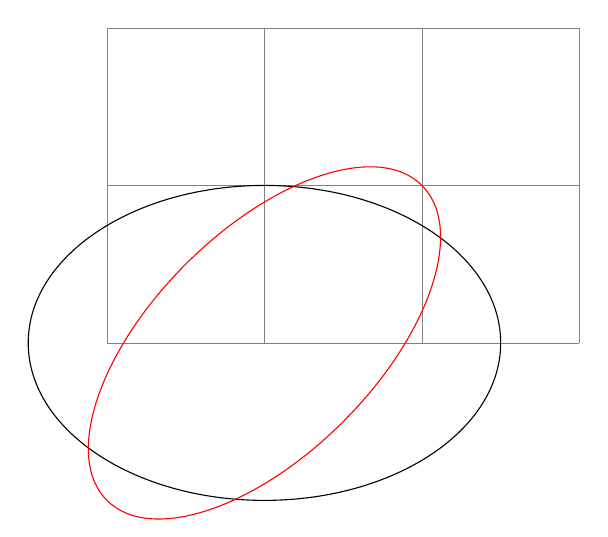
\begin{tikzpicture}[scale=2]
  \draw[help lines] (0,0) grid (3,2);
  \pgfpathellipse{\pgfpoint{1cm}{0cm}}{\pgfpoint{1.5cm}{0cm}}{\pgfpoint{0cm}{1cm}}
  \pgfusepath{draw}
  \color{red}
  \pgfpathellipse{\pgfpoint{1cm}{0cm}}{\pgfpoint{1cm}{1cm}}{\pgfpoint{-0.5cm}{0.5cm}}
  \pgfusepath{draw}
\end{tikzpicture}

rectangle:
\begin{tikzpicture}[scale=2]
  \draw[help lines] (0,0) grid (3,2);
  \pgfpathrectangle{\pgfpoint{1cm}{0cm}}{\pgfpoint{1.5cm}{1cm}}
  \pgfpathrectangle{\pgfpoint{1.5cm}{0.25cm}}{\pgfpoint{1.5cm}{1cm}}
  \pgfpathrectangle{\pgfpoint{2cm}{0.5cm}}{\pgfpoint{1.5cm}{1cm}}
  \pgfusepath{draw}
\end{tikzpicture}

grid
\begin{pgfpicture}[scale=2]
  \pgfsetlinewidth{0.8pt}
  \pgfpathgrid[step={\pgfpoint{1cm}{1cm}}]{\pgfpoint{-3mm}{-3mm}}{\pgfpoint{33mm}{23mm}}
  \pgfusepath{stroke}
  \pgfsetlinewidth{0.4pt}
  \pgfpathgrid[stepx=1mm,stepy=1mm]{\pgfpoint{-1.5mm}{-1.5mm}}{\pgfpoint{31.5mm}{21.5mm}}
  \pgfusepath{stroke}
\end{pgfpicture}

pgfpathparabola:
\begin{pgfpicture}[scale=2]
  % Half-parabola going ‘‘up and right’’
  \pgfpathmoveto{\pgfpointorigin}
  \pgfpathparabola{\pgfpointorigin}{\pgfpoint{2cm}{4cm}}
  \color{red}
  \pgfusepath{stroke}
  % Half-parabola going ‘‘down and right’’
  \pgfpathmoveto{\pgfpointorigin}
  \pgfpathparabola{\pgfpoint{-2cm}{4cm}}{\pgfpointorigin}
  \color{blue}
  \pgfusepath{stroke}
  % Full parabola
  \pgfpathmoveto{\pgfpoint{-2cm}{2cm}}
  \pgfpathparabola{\pgfpoint{1cm}{-1cm}}{\pgfpoint{2cm}{4cm}}
  \color{orange}
  \pgfusepath{stroke}
\end{pgfpicture}

sine, cosine:
\begin{tikzpicture}[scale=2]
  \draw[help lines] (0,0) grid (3,1);
  \pgfpathmoveto{\pgfpoint{1cm}{0cm}}
  \pgfpathsine{\pgfpoint{1cm}{1cm}}
  \pgfusepath{stroke}
  \color{red}
  \pgfpathmoveto{\pgfpoint{1cm}{0cm}}
  \pgfpathsine{\pgfpoint{-2cm}{-2cm}}
  \pgfusepath{stroke}
\end{tikzpicture}
\begin{pgfpicture}[scale=2]
  \pgfpathmoveto{\pgfpoint{0cm}{0cm}}
  \pgfpathsine{\pgfpoint{1cm}{1cm}}
  \pgfpathcosine{\pgfpoint{1cm}{-1cm}}
  \pgfpathsine{\pgfpoint{1cm}{-1cm}}
  \pgfpathcosine{\pgfpoint{1cm}{1cm}}
  % Something is wrong with the "svg brown"
  \pgfsetfillcolor{brown}
  \pgfusepath{fill,stroke}
\end{pgfpicture}

% plots - see plots
rounded corners
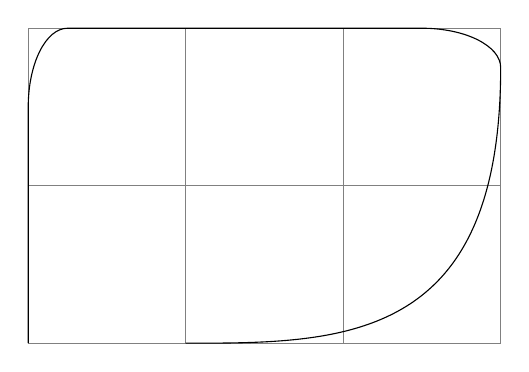
\begin{tikzpicture}[scale=2]
  \draw[help lines] (0,0) grid (3,2);
  \pgfsetcornersarced{\pgfpoint{10mm}{5mm}}
  % 10mm entering,
  % 5mm leaving.
  \pgfpathmoveto{\pgfpointorigin}
  \pgfpathlineto{\pgfpoint{0cm}{2cm}}
  \pgfpathlineto{\pgfpoint{3cm}{2cm}}
  \pgfpathcurveto{\pgfpoint{3cm}{0cm}}{\pgfpoint{2cm}{0cm}}{\pgfpoint{1cm}{0cm}}
  \pgfusepath{stroke}
\end{tikzpicture}
\begin{pgfpicture}[scale=2]
  \pgfsetcornersarced{\pgfpoint{4pt}{4pt}}
  \pgfpathmoveto{\pgfpointpolar{0}{1cm}}
  \pgfpathlineto{\pgfpointpolar{72}{1cm}}
  \pgfpathlineto{\pgfpointpolar{144}{1cm}}
  \pgfpathlineto{\pgfpointpolar{216}{1cm}}
  \pgfpathlineto{\pgfpointpolar{288}{1cm}}
  \pgfpathclose
  \pgfusepath{stroke}
\end{pgfpicture}
\endgroup % ----------- end -----------------
%======================================================================
\section{Decorations}
\begingroup % ------ pseudo document ---------
\tikz \draw decorate[decoration=zigzag] {(0,0) -- (3,0)};
\endgroup % ----------- end -----------------

\begingroup % ------ pseudo document ---------
% TODO: stuck in loop; (Deep recursion in dimensions?)
%%\tikz \fill [decorate,decoration={text along path,
%%   text=This is a text along a path. Note how the path}]
%%  [fill=blue!20,draw=blue,thick] (0,0) -- (2,1) arc (90:-90:.5) -- cycle;

% pgfdeclaredecoration
\pgfdeclaredecoration{example}{initial}{
  \state{initial}[width=10pt]{
    \pgfpathlineto{\pgfpoint{0pt}{5pt}}
    \pgfpathlineto{\pgfpoint{5pt}{5pt}}
    \pgfpathlineto{\pgfpoint{5pt}{-5pt}}
    \pgfpathlineto{\pgfpoint{10pt}{-5pt}}
    \pgfpathlineto{\pgfpoint{10pt}{0pt}}
  }
  \state{final}{
    \pgfpathlineto{\pgfpointdecoratedpathlast}
  }
}
\tikz[decoration=example]{
  \draw [decorate] (0,0) -- (3,0);
  \draw [red,decorate] (0,0) to [out=45,in=135] (3,0);
}
\pgfdeclaredecoration{stars}{initial}{
  \state{initial}[width=15pt]{
    \pgfmathparse{round(rnd*100)}
    \pgfsetfillcolor{yellow!\pgfmathresult!orange}
    \pgfsetstrokecolor{yellow!\pgfmathresult!red}
    \pgfnode{star}{center}{}{}{\pgfusepath{stroke,fill}}
  }
  \state{final}{
    \pgfpathmoveto{\pgfpointdecoratedpathlast}
  }
}
\tikz\path[decorate, decoration=stars, star point ratio=2, star points=5,
    inner sep=0, minimum size=rnd*10pt+2pt]
  (0,0) .. controls (0,2) and (3,2) .. (3,0)
  .. controls (3,-3) and (0,0) .. (0,-3)
  .. controls (0,-5) and (3,-5) .. (3,-3);
  \pgfdeclaredecoration{complicated example decoration}{initial}{
    \state{initial}[width=5pt,next state=up]{
       \pgfpathlineto{\pgfpoint{5pt}{0pt}} }
    \state{up}[width=5pt,next state=down]{
       \ifdim\pgfdecoratedremainingdistance>\pgfdecoratedcompleteddistance
         % Growing
         \pgfpathlineto{\pgfpoint{0pt}{\pgfdecoratedcompleteddistance}}
         \pgfpathlineto{\pgfpoint{5pt}{\pgfdecoratedcompleteddistance}}
         \pgfpathlineto{\pgfpoint{5pt}{0pt}}
       \else
         % Shrinking
         \pgfpathlineto{\pgfpoint{0pt}{\pgfdecoratedremainingdistance}}
         \pgfpathlineto{\pgfpoint{5pt}{\pgfdecoratedremainingdistance}}
         \pgfpathlineto{\pgfpoint{5pt}{0pt}}
        \fi}
     \state{down}[width=5pt,next state=up]{
       \ifdim\pgfdecoratedremainingdistance>\pgfdecoratedcompleteddistance
         % Growing
         \pgfpathlineto{\pgfpoint{0pt}{-\pgfdecoratedcompleteddistance}}
         \pgfpathlineto{\pgfpoint{5pt}{-\pgfdecoratedcompleteddistance}}
         \pgfpathlineto{\pgfpoint{5pt}{0pt}}
       \else
         % Shrinking
         \pgfpathlineto{\pgfpoint{0pt}{-\pgfdecoratedremainingdistance}}
         \pgfpathlineto{\pgfpoint{5pt}{-\pgfdecoratedremainingdistance}}
         \pgfpathlineto{\pgfpoint{5pt}{0pt}}
       \fi}
     \state{final}{
       \pgfpathlineto{\pgfpointdecoratedpathlast}
     }
   }
\begin{tikzpicture}[decoration=complicated example decoration]
  \draw decorate{ (0,0) -- (3,0)};
  \fill [red!50,rounded corners=2pt]
  decorate {(.5,-2) -- ++(2.5,-2.5)} -- (3,-5) -| (0,-2) -- cycle;
\end{tikzpicture}
%\catcode`\|12
%\begin{tikzpicture}
%\draw [help lines] grid (3,2);
%\fill [draw=red,fill=red!20,
%postaction={decorate,decoration={raise=2pt,text along path,
%text=around and around and around and around we go}}]
%(0,1) arc (180:-180:1.5cm and 1cm);
%\end{tikzpicture}

\endgroup % ----------- end -----------------
%======================================================================
\section{More Paths}
% TODO: xlink:href; clipped path (last)
% TODO: arrows
\begingroup % ------ pseudo document ---------
% pgfusepath
fill, stroke
\begin{pgfpicture}[scale=2]
  \pgfpathmoveto{\pgfpointorigin}
  \pgfpathlineto{\pgfpoint{1cm}{1cm}}
  \pgfpathlineto{\pgfpoint{1cm}{0cm}}
  \pgfusepath{fill}
\end{pgfpicture}
\begin{pgfpicture}[scale=2]
  \pgfpathmoveto{\pgfpointorigin}
  \pgfpathlineto{\pgfpoint{1cm}{1cm}}
  \pgfpathlineto{\pgfpoint{1cm}{0cm}}
  \pgfusepath{stroke}
\end{pgfpicture}

clip
\begin{pgfpicture}[scale=2]
  \pgfpathmoveto{\pgfpointorigin}
  \pgfpathlineto{\pgfpoint{1cm}{1cm}}
  \pgfpathlineto{\pgfpoint{1cm}{0cm}}
  \pgfusepath{stroke,clip}
  \pgfpathcircle{\pgfpoint{1cm}{1cm}}{0.5cm}
  \pgfusepath{fill}
\end{pgfpicture}
% pgfsetlinewidth
\begin{pgfpicture}[scale=2]
  \pgfsetlinewidth{1mm}
  \pgfpathmoveto{\pgfpoint{0mm}{0mm}}
  \pgfpathlineto{\pgfpoint{2cm}{0mm}}
  \pgfusepath{stroke}
  \pgfsetlinewidth{2\pgflinewidth} % double in size
  \pgfpathmoveto{\pgfpoint{0mm}{5mm}}
  \pgfpathlineto{\pgfpoint{2cm}{5mm}}
  \pgfusepath{stroke}
\end{pgfpicture}
% pgfsetstrokecolor
\begin{pgfpicture}[scale=2]
  \pgfsetlinewidth{1pt}
  \color{red}
  \pgfpathcircle{\pgfpoint{0cm}{0cm}}{3mm} \pgfusepath{fill,stroke}
  \pgfsetstrokecolor{black}
  \pgfpathcircle{\pgfpoint{1cm}{0cm}}{3mm} \pgfusepath{fill,stroke}
  \color{red}
  \pgfpathcircle{\pgfpoint{2cm}{0cm}}{3mm} \pgfusepath{fill,stroke}
\end{pgfpicture}
% arrows
\begin{pgfpicture}[scale=2]
  \pgfsetarrowsstart{latex}
  \pgfsetarrowsend{to}
  \pgfpathmoveto{\pgfpointorigin}
  \pgfpathlineto{\pgfpoint{1cm}{0cm}}
  \pgfusepath{stroke}
\end{pgfpicture}
%
% Filling a path
%
% pgfseteorule
\begin{pgfpicture}[scale=2]
  \pgfseteorule
  \pgfpathcircle{\pgfpoint{0mm}{0cm}}{7mm}
  \pgfpathcircle{\pgfpoint{5mm}{0cm}}{7mm}
  \pgfusepath{fill}
\end{pgfpicture}
% pgfsetnonzerorule
\begin{pgfpicture}[scale=2]
  \pgfsetnonzerorule
  \pgfpathcircle{\pgfpoint{0mm}{0cm}}{7mm}
  \pgfpathcircle{\pgfpoint{5mm}{0cm}}{7mm}
  \pgfusepath{fill}
\end{pgfpicture}\\
%
% Using a path as a bounding box
%
\begin{pgfpicture}[scale=2]
  \pgfpathrectangle{\pgfpointorigin}{\pgfpoint{2ex}{1ex}}
  \pgfusepath{use as bounding box} % draws nothing
  \pgfpathcircle{\pgfpointorigin}{2ex}
  \pgfusepath{stroke}
\end{pgfpicture}% right.

\endgroup % ----------- end -----------------
%======================================================================
\section{Arrows}

\begingroup % ------ pseudo document ---------
\begin{pgfpicture}
  \pgfsetarrowsstart{latex}
  \pgfsetarrowsend{to}
  \pgfpathmoveto{\pgfpointorigin}
  \pgfpathlineto{\pgfpoint{1cm}{0cm}}
  \pgfusepath{stroke}
\end{pgfpicture}
%
% Declaring an arrow tip kind
%
\pgfarrowsdeclare{arcs’’}{arcs’’}{
  \arrowsize=0.2pt
  \advance\arrowsize by .5\pgflinewidth
  \pgfarrowsleftextend{-4\arrowsize-.5\pgflinewidth}
  \pgfarrowsrightextend{.5\pgflinewidth}
  }
  {
  \arrowsize=0.2pt
  \advance\arrowsize by .5\pgflinewidth
  \pgfsetdash{}{0pt} % do not dash
  \pgfsetroundjoin
  % fix join
  \pgfsetroundcap
  % fix cap
  \pgfpathmoveto{\pgfpoint{-4\arrowsize}{4\arrowsize}}
  \pgfpatharc{180}{270}{4\arrowsize}
  \pgfusepathqstroke
  \pgfpathmoveto{\pgfpointorigin}
  \pgfpatharc{90}{180}{4\arrowsize}
  \pgfusepathqstroke
}

%%% Something wrong with -arcs'' ???
% \begin{tikzpicture}[scale=2]
% \draw[help lines] (-2,-1) grid (1,1);
% \draw[line width=10pt,-arcs’’] (-2,0) -- (0,0);
% \draw[line width=2pt,white] (-2,0) -- (0,0);
% \end{tikzpicture}

%
% Declaring a dertived arrow tip kind
%
% pgfarrowsdeclarealias
\pgfarrowsdeclarealias{<}{>}{arcs’’}{arcs’’}%
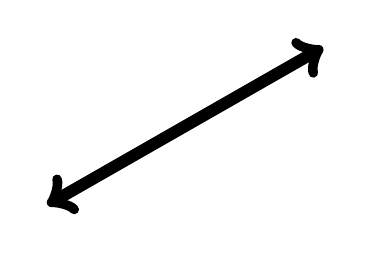
\begin{tikzpicture}
  \pgfsetarrows{<->}
  \pgfsetlinewidth{1ex}
  \pgfpathmoveto{\pgfpointorigin}
  \pgfpathlineto{\pgfpoint{3.5cm}{2cm}}
  \pgfusepath{stroke}
  \useasboundingbox (-0.25,-0.25) rectangle (3.75,2.25);
\end{tikzpicture}
% pgfarrowsdeclarereversed
\pgfarrowsdeclarereversed{arcs reversed}{arcs reversed}{arcs’’}{arcs’’}%
\begin{tikzpicture}
  \pgfsetarrows{arcs reversed-arcs reversed}
  \pgfsetlinewidth{1ex}
  \pgfpathmoveto{\pgfpointorigin}
  \pgfpathlineto{\pgfpoint{3.5cm}{2cm}}
  \pgfusepath{stroke}
  \useasboundingbox (-0.25,-0.25) rectangle (3.75,2.25);
\end{tikzpicture}
% pgfarrowsdeclarecombined
\pgfarrowsdeclarecombine[\pgflinewidth]{combined}{combined}{arcs’’}{arcs’’}{latex}{latex}%
\begin{tikzpicture}
  \pgfsetarrows{combined-combined}
  \pgfsetlinewidth{1ex}
  \pgfpathmoveto{\pgfpointorigin}
  \pgfpathlineto{\pgfpoint{3.5cm}{2cm}}
  \pgfusepath{stroke}
  \useasboundingbox (-0.25,-0.25) rectangle (3.75,2.25);
\end{tikzpicture}
\pgfarrowsdeclarecombine*[\pgflinewidth]{combined’}{combined’}{arcs’’}{arcs’’}{latex}{latex}%
% Something wrong here too
% \begin{tikzpicture}
% \pgfsetarrows{combined’-combined’}
% \pgfsetlinewidth{1ex}
% \pgfpathmoveto{\pgfpointorigin}
% \pgfpathlineto{\pgfpoint{3.5cm}{2cm}}
% \pgfusepath{stroke}
% \useasboundingbox (-0.25,-0.25) rectangle (3.75,2.25);
% \end{tikzpicture}
% pgfarrowsdeclaretriple
\pgfarrowsdeclaretriple{<<<}{>>>}{arcs’’}{arcs’’}%
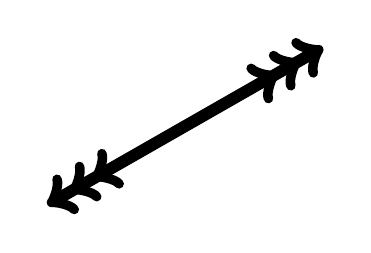
\begin{tikzpicture}
  \pgfsetarrows{<<<->>>}
  \pgfsetlinewidth{1ex}
  \pgfpathmoveto{\pgfpointorigin}
  \pgfpathlineto{\pgfpoint{3.5cm}{2cm}}
  \pgfusepath{stroke}
  \useasboundingbox (-0.25,-0.25) rectangle (3.75,2.25);
\end{tikzpicture}
%
% Using an arrow tip kind
%
% pgfsetarrowsstart
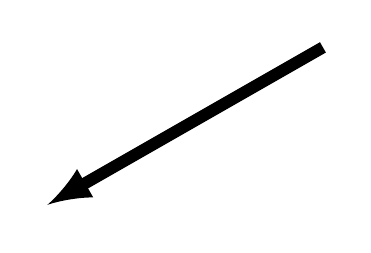
\begin{tikzpicture}
  \pgfsetarrowsstart{latex}
  \pgfsetlinewidth{1ex}
  \pgfpathmoveto{\pgfpointorigin}
  \pgfpathlineto{\pgfpoint{3.5cm}{2cm}}
  \pgfusepath{stroke}
  \useasboundingbox (-0.25,-0.25) rectangle (3.75,2.25);
\end{tikzpicture}
% pgfsetarrowsend
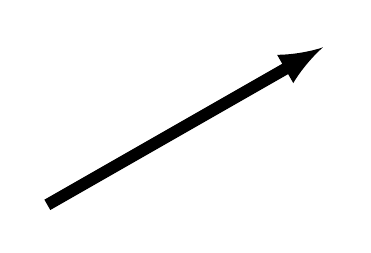
\begin{tikzpicture}
  \pgfsetarrowsend{latex}
  \pgfsetlinewidth{1ex}
  \pgfpathmoveto{\pgfpointorigin}
  \pgfpathlineto{\pgfpoint{3.5cm}{2cm}}
  \pgfusepath{stroke}
  \useasboundingbox (-0.25,-0.25) rectangle (3.75,2.25);
\end{tikzpicture}
% pgfsetarrows
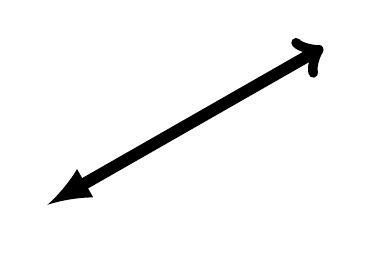
\begin{tikzpicture}
  \pgfsetarrows{latex-to}
  \pgfsetlinewidth{1ex}
  \pgfpathmoveto{\pgfpointorigin}
  \pgfpathlineto{\pgfpoint{3.5cm}{2cm}}
  \pgfusepath{stroke}
  \useasboundingbox (-0.25,-0.25) rectangle (3.75,2.25);
\end{tikzpicture}
\endgroup % ----------- end -----------------
%======================================================================
\section{Nodes}
% TODO: Fadings
% TODO: Color in box
% TODO: arrows
\begingroup % ------ pseudo document ---------
\catcode`\@=11\relax
\pgfdeclareshape{document}{
\inheritsavedanchors[from=rectangle] % this is nearly a rectangle
\inheritanchorborder[from=rectangle]
\inheritanchor[from=rectangle]{center}
\inheritanchor[from=rectangle]{north}
\inheritanchor[from=rectangle]{south}
\inheritanchor[from=rectangle]{west}
\inheritanchor[from=rectangle]{east}
% ... and possibly more
\backgroundpath{% this is new
% store lower right in xa/ya and upper right in xb/yb
\southwest \pgf@xa=\pgf@x \pgf@ya=\pgf@y
\northeast \pgf@xb=\pgf@x \pgf@yb=\pgf@y
% compute corner of ‘‘flipped page’’
\pgf@xc=\pgf@xb \advance\pgf@xc by-5pt % this should be a parameter
\pgf@yc=\pgf@yb \advance\pgf@yc by-5pt
% construct main path
\pgfpathmoveto{\pgfpoint{\pgf@xa}{\pgf@ya}}
\pgfpathlineto{\pgfpoint{\pgf@xa}{\pgf@yb}}
\pgfpathlineto{\pgfpoint{\pgf@xc}{\pgf@yb}}
\pgfpathlineto{\pgfpoint{\pgf@xb}{\pgf@yc}}
\pgfpathlineto{\pgfpoint{\pgf@xb}{\pgf@ya}}
\pgfpathclose
% add little corner
\pgfpathmoveto{\pgfpoint{\pgf@xc}{\pgf@yb}}
\pgfpathlineto{\pgfpoint{\pgf@xc}{\pgf@yc}}
\pgfpathlineto{\pgfpoint{\pgf@xb}{\pgf@yc}}
\pgfpathlineto{\pgfpoint{\pgf@xc}{\pgf@yc}}
}
}\hskip-1.2cm
\begin{tikzpicture}
  \node[shade,draw,shape=document,inner sep=2ex] (x) {Remark};
  \node[fill=olive,draw,ellipse,double]
  at ([shift=(-80:3cm)]x) (y) {Use Case};
  \draw[dashed] (x) -- (y);
\end{tikzpicture}

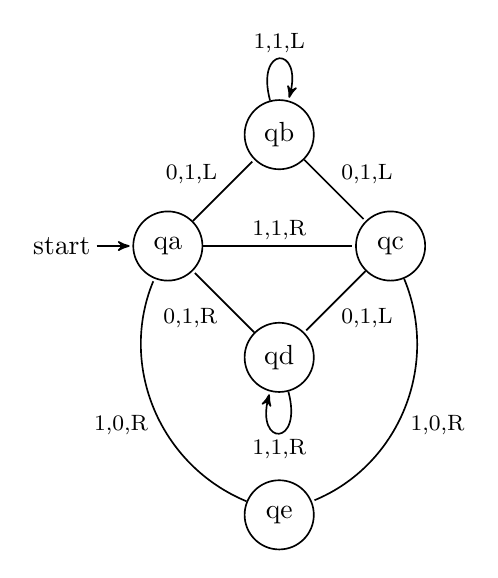
\begin{tikzpicture}[>=stealth',shorten >=1pt,%
    auto,node distance=2cm,on grid,semithick,
    inner sep=2pt,bend angle=45]
  \node[initial,state] (A) {qa};
  \node[state] (B) [above right=of A] {qb};
  \node[state] (D) [below right=of A] {qd};
  \node[state] (C) [below right=of B] {qc};
  \node[state] (E) [below=of D] {qe};

  \path [every node/.style={font=\footnotesize}]
    (A) edge node {0,1,L} (B) edge node {1,1,R} (C)
    (B) edge [loop above] node {1,1,L} (B) edge node {0,1,L} (C)
    (C) edge node {0,1,L} (D) edge [bend left] node {1,0,R} (E)
    (D) edge [loop below] node {1,1,R} (D) edge node {0,1,R} (A)
    (E) edge [bend left] node {1,0,R} (A);
\end{tikzpicture}

\endgroup % ----------- end -----------------

\begingroup % ------ pseudo document ---------
%
% Creating nodes
%
% pgfnode
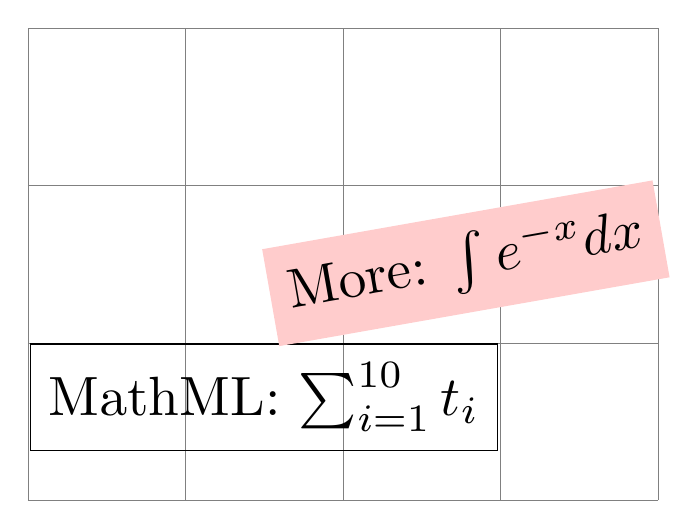
\begin{tikzpicture}[scale=2]
  \draw[help lines] (0,0) grid (4,3);
   {
     \pgftransformshift{\pgfpoint{1.5cm}{1cm}}
     \pgfnode{rectangle}{north}{MathML: $\sum_{i=1}^{10} t_i$}{hellonode}{\pgfusepath{stroke}}
   }
   {
     \color{red!20}
     \pgftransformrotate{10}
     \pgftransformshift{\pgfpoint{3cm}{1cm}}
     \pgfnode{rectangle}{center}{\color{black}More: $\int e^{-x}dx$}{hellonode}{\pgfusepath{fill}}
   }
\end{tikzpicture}

% pgftransformresetnontranslations
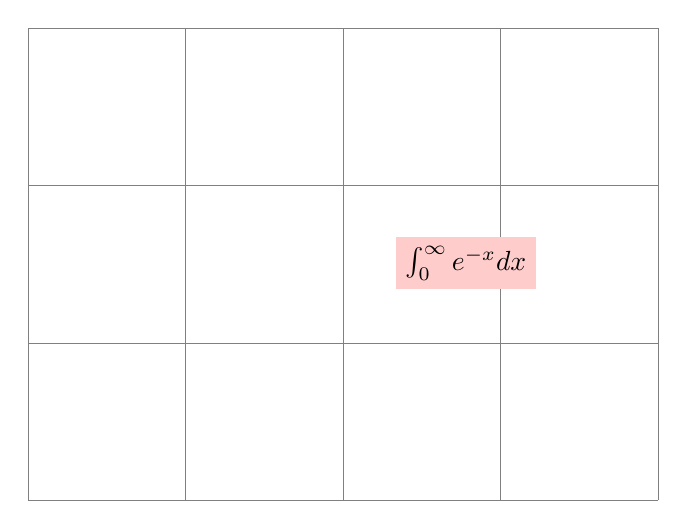
\begin{tikzpicture}[scale=2]
  \draw[help lines] (0,0) grid (4,3);
  {
    \color{red!20}
    \pgftransformrotate{10}
    \pgftransformshift{\pgfpoint{3cm}{1cm}}
    \pgftransformresetnontranslations
    \pgfnode{rectangle}{center}{\color{black}$\int_0^\infty e^{-x}dx$}{hellonode}{\pgfusepath{fill}}
  }
\end{tikzpicture}
% pgfmultipartnode
\setbox\pgfnodeparttextbox=\hbox{q}
\setbox\pgfnodepartlowerbox=\hbox{01}
\begin{pgfpicture}[scale=2]
  \pgfmultipartnode{circle split}{center}{my state}{\pgfusepath{stroke}}
\end{pgfpicture}
%  different keys
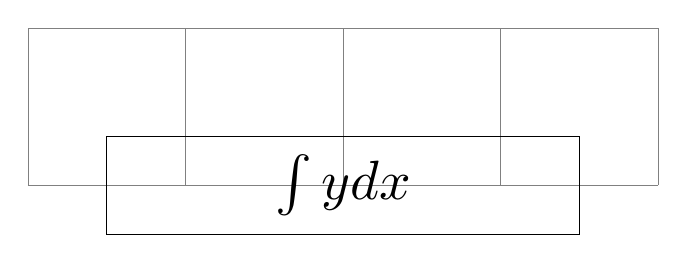
\begin{tikzpicture}[scale=2]
  \draw[help lines] (-2,0) grid (2,1);
  \pgfset{minimum width=3cm}
  \pgfnode{rectangle}{center}{$\int y dx$}{}{\pgfusepath{stroke}}
\end{tikzpicture}
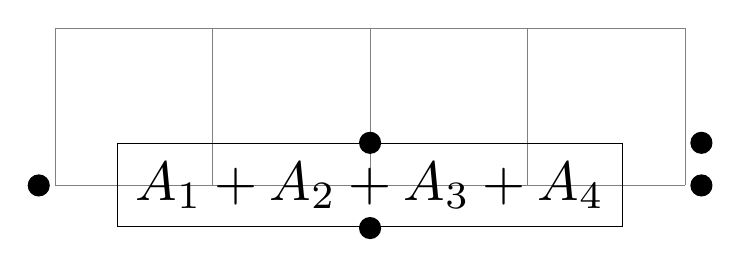
\begin{tikzpicture}[scale=2]
  \draw[help lines] (-2,0) grid (2,1);
  \pgfset{outer xsep=.5cm}
  \pgfnode{rectangle}{center}{$A_1+A_2+A_3+A_4$}{x}{\pgfusepath{stroke}}
  \pgfpathcircle{\pgfpointanchor{x}{north}}{2pt}
  \pgfpathcircle{\pgfpointanchor{x}{south}}{2pt}
  \pgfpathcircle{\pgfpointanchor{x}{east}}{2pt}
  \pgfpathcircle{\pgfpointanchor{x}{west}}{2pt}
  \pgfpathcircle{\pgfpointanchor{x}{north east}}{2pt}
  \pgfusepath{fill}
\end{tikzpicture}
%
% Using anchors
%
% pgfpointanchor
\begin{pgfpicture}[scale=2]
  \pgftransformrotate{30}
  \pgfnode{rectangle}{center}{Hello World!}{x}{\pgfusepath{stroke}}
  \pgfpathcircle{\pgfpointanchor{x}{north}}{2pt}
  \pgfpathcircle{\pgfpointanchor{x}{south}}{2pt}
  \pgfpathcircle{\pgfpointanchor{x}{east}}{2pt}
  \pgfpathcircle{\pgfpointanchor{x}{west}}{2pt}
  \pgfpathcircle{\pgfpointanchor{x}{north east}}{2pt}
  \pgfusepath{fill}
\end{pgfpicture}
% pgfpointshapeborder
\begin{pgfpicture}[scale=2]
  \begin{pgfscope}
    \pgftransformrotate{30}
    \pgfnode{rectangle}{center}{Hello World!}{x}{\pgfusepath{stroke}}
  \end{pgfscope}
  \pgfpathcircle{\pgfpointshapeborder{x}{\pgfpoint{2cm}{1cm}}}{2pt}
  \pgfpathcircle{\pgfpoint{2cm}{1cm}}{2pt}
  \pgfpathcircle{\pgfpointshapeborder{x}{\pgfpoint{-1cm}{1cm}}}{2pt}
  \pgfpathcircle{\pgfpoint{-1cm}{1cm}}{2pt}
  \pgfusepath{fill}
\end{pgfpicture}
\endgroup % ----------- end -----------------
%======================================================================
\section{Matrices}
\begingroup % ------ pseudo document ---------
%
% pgfmatrix command
%
\newbox\foo\setbox\foo=\hbox{a}
\begin{tikzpicture}
  \pgfmatrix{rectangle}{center}{mymatrix}{\pgfusepath{}}{\pgfpointorigin}{}
  {
    \node{a};\pgfmatrixendrow
  }
\end{tikzpicture}
\endgroup % ----------- end -----------------
%======================================================================
\section{Transformations}
\begingroup % ------ pseudo document ---------
%
% Canvas transformation
%
% pgflowlevelsynccm
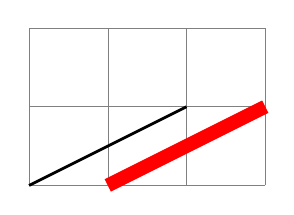
\begin{tikzpicture}
  \draw[help lines] (0,0) grid (3,2);
  \pgfsetlinewidth{1pt}
  \pgftransformscale{5}
  \draw (0,0) -- (0.4,.2);
  \pgftransformxshift{0.2cm}
  \pgflowlevelsynccm
  \draw[red] (0,0) -- (0.4,.2);
\end{tikzpicture}
% pgflowlevel
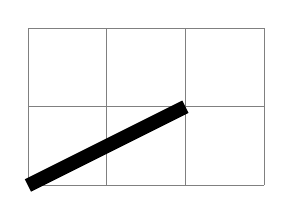
\begin{tikzpicture}
  \draw[help lines] (0,0) grid (3,2);
  \pgfsetlinewidth{1pt}
  \pgflowlevel{\pgftransformscale{5}}
  \draw (0,0) -- (0.4,.2);
\end{tikzpicture}
% pgflowlevelobj
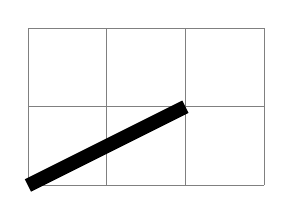
\begin{tikzpicture}
  \draw[help lines] (0,0) grid (3,2);
  \pgfsetlinewidth{1pt}
  \pgflowlevelobj{\pgftransformscale{5}}
  {\draw (0,0) -- (0.4,.2);}
  \pgflowlevelobj{\pgftransformxshift{-1cm}}{\draw (0,0) -- (0.4,.2);}
\end{tikzpicture}
% pgflowlevelscope
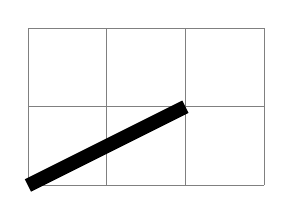
\begin{tikzpicture}
  \draw[help lines] (0,0) grid (3,2);
  \pgfsetlinewidth{1pt}
  \begin{pgflowlevelscope}{\pgftransformscale{5}}
    \draw (0,0) -- (0.4,.2);
  \end{pgflowlevelscope}
  \begin{pgflowlevelscope}{\pgftransformxshift{-1cm}}
    \draw (0,0) -- (0.4,.2);
  \end{pgflowlevelscope}
\end{tikzpicture}
\endgroup % ----------- end -----------------

% TODO: Weird placement of text
\begingroup % ------ pseudo document ---------
%
% Coordinate transformation
%
% pgftransformshift
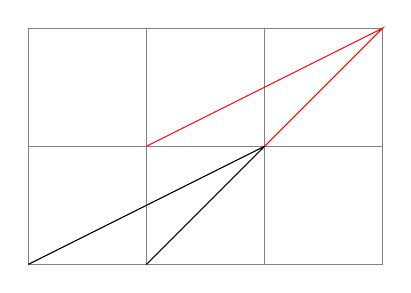
\begin{tikzpicture}[scale=1.5]
  \draw[help lines] (0,0) grid (3,2);
  \draw (0,0) -- (2,1) -- (1,0);
  \pgftransformshift{\pgfpoint{1cm}{1cm}}
  \draw[red] (0,0) -- (2,1) -- (1,0);
\end{tikzpicture}
% pgftransformscale
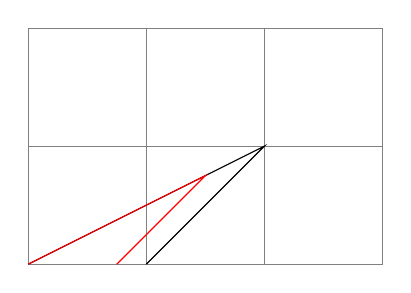
\begin{tikzpicture}[scale=1.5]
  \draw[help lines] (0,0) grid (3,2);
  \draw (0,0) -- (2,1) -- (1,0);
  \pgftransformscale{.75}
  \draw[red] (0,0) -- (2,1) -- (1,0);
\end{tikzpicture}

% pgftransformxslant
\begin{tikzpicture}
  \draw[help lines] (0,0) grid (3,2);
  \draw (0,0) -- (2,1) -- (1,0);
  \pgftransformxslant{.5}
  \draw[red] (0,0) -- (2,1) -- (1,0);
\end{tikzpicture}
% pgftransformrotate
\begin{tikzpicture}
  \draw[help lines] (0,0) grid (3,2);
  \draw (0,0) -- (2,1) -- (1,0);
  \pgftransformrotate{30}
  \draw[red] (0,0) -- (2,1) -- (1,0);
\end{tikzpicture}

% pgftransformtriangle
\begin{tikzpicture}
  \draw[help lines] (0,0) grid (3,2);
  \pgftransformtriangle
    {\pgfpoint{1cm}{0cm}}
    {\pgfpoint{0cm}{2cm}}
    {\pgfpoint{3cm}{1cm}}
  \draw (0,0) -- (1pt,0pt) -- (0pt,1pt) -- cycle;
\end{tikzpicture}
% pgftransformcm
\begin{tikzpicture}
  \draw[help lines] (0,0) grid (3,2);
  \draw (0,0) -- (2,1) -- (1,0);
  \pgftransformcm{1}{1}{0}{1}{\pgfpoint{.25cm}{.25cm}}
  \draw[red] (0,0) -- (2,1) -- (1,0);
\end{tikzpicture}
% pgftransformarrow
\begin{tikzpicture}
  \draw[help lines] (0,0) grid (3,2);
  \draw (0,0) -- (3,1);
  \pgftransformarrow{\pgfpointorigin}{\pgfpoint{3cm}{1cm}}
  \pgftext{tip}
\end{tikzpicture}

% pgftransformcurveattime
\begin{tikzpicture}
  \draw[help lines] (0,0) grid (3,2);
  \draw (0,0) .. controls (0,2) and (1,2) .. (2,1);
  \pgfslopedattimetrue
  \pgftransformcurveattime{.25}{\pgfpointorigin}
    {\pgfpoint{0cm}{2cm}}{\pgfpoint{1cm}{2cm}}{\pgfpoint{2cm}{1cm}}
  \pgftext{Hi!}
\end{tikzpicture}
% pgftransformreset
\begin{tikzpicture}
  \draw[help lines] (0,0) grid (3,2);
  \pgftransformrotate{30}
  \draw (0,0) -- (2,1) -- (1,0);
  \pgftransformreset
  \draw[red] (0,0) -- (2,1) -- (1,0);
\end{tikzpicture}
%pgftransformresetnontranslations
\begin{tikzpicture}
  \draw[help lines] (0,0) grid (3,2);
  \pgftransformscale{2}
  \pgftransformrotate{30}
  \pgftransformxshift{1cm}{\color{red}\pgftext{rotated}}
  \pgftransformresetnontranslations
  \pgftext{shifted only}
\end{tikzpicture}
% pgftransforminvert
\begin{tikzpicture}
  \draw[help lines] (0,0) grid (3,2);
  \pgftransformrotate{30}
  \draw (0,0) -- (2,1) -- (1,0);
  \pgftransforminvert
  \draw[red] (0,0) -- (2,1) -- (1,0);
\end{tikzpicture}
\endgroup % ----------- end -----------------
%======================================================================
\section{Patterns}
% TODO: Centos6 tikz XKeyVal
\begingroup % ------ pseudo document ---------
%
% Declaring a pattern
%
% pgfdeclarepatternformonly
\pgfdeclarepatternformonly{stars}
  {\pgfpointorigin}{\pgfpoint{1cm}{1cm}}
  {\pgfpoint{1cm}{1cm}}
  {
    \pgftransformshift{\pgfpoint{.5cm}{.5cm}}
    \pgfpathmoveto{\pgfpointpolar{0}{4mm}}
    \pgfpathlineto{\pgfpointpolar{144}{4mm}}
    \pgfpathlineto{\pgfpointpolar{288}{4mm}}
    \pgfpathlineto{\pgfpointpolar{72}{4mm}}
    \pgfpathlineto{\pgfpointpolar{216}{4mm}}
    \pgfpathclose%
    \pgfusepath{fill}
  }
\begin{tikzpicture}
  \filldraw[pattern=stars] (0,0) rectangle (1.5,2);
  \filldraw[pattern=stars,pattern color=red] (1.5,0) rectangle (3,2);
\end{tikzpicture}

% pgfdeclarepatterninherentlycolored
\pgfdeclarepatterninherentlycolored{green stars}
  {\pgfpointorigin}{\pgfpoint{1cm}{1cm}}
  {\pgfpoint{1cm}{1cm}}
  {
    \pgfsetfillcolor{green!50!black}
    \pgftransformshift{\pgfpoint{.5cm}{.5cm}}
    \pgfpathmoveto{\pgfpointpolar{0}{4mm}}
    \pgfpathlineto{\pgfpointpolar{144}{4mm}}
    \pgfpathlineto{\pgfpointpolar{288}{4mm}}
    \pgfpathlineto{\pgfpointpolar{72}{4mm}}
    \pgfpathlineto{\pgfpointpolar{216}{4mm}}
    \pgfpathclose%
    \pgfusepath{stroke,fill}
  }
\begin{tikzpicture}
  \filldraw[pattern=green stars] (0,0) rectangle (3,2);
\end{tikzpicture}

% Setting a pattern
%
% pgfsetfillpattern
\begin{tikzpicture}
  \pgfsetfillpattern{stars}{red} \filldraw (0,0) rectangle (1.5,2);
  \pgfsetfillpattern{green stars}{red} \filldraw (1.5,0) rectangle (3,2);
\end{tikzpicture}
\endgroup % ----------- end -----------------
%======================================================================
\section{Plots}
\begingroup % ------ pseudo document ---------
% pgfplotstream(start|point|end)
\begin{tikzpicture}
  \pgfplothandlerlineto
  \pgfplotstreamstart
  \pgfplotstreampoint{\pgfpointxyz{2}{-5}{1}}
  \pgfplotstreampoint{\pgfpointxyz{2}{-.2}{2}}
  \pgfplotstreampoint{\pgfpointxyz{2}{-5}{2}}
  \pgfplotstreamend
  \pgfusepath{stroke}
\end{tikzpicture}
%
% Generating plot streams
%
% pgfplotxyfile
% pgfplotxyzfile
% pgfplotfunction
\begin{tikzpicture}[x=3.8cm/360]
  \pgfplothandlerlineto
  \pgfplotfunction{\x}{0,5,...,360}{\pgfpointxy{\x}{sin(\x)+sin(3*\x)}}
  \pgfusepath{stroke}
\end{tikzpicture}
\begin{tikzpicture}[y=3cm/360]
  \pgfplothandlerlineto
  \pgfplotfunction{\y}{0,5,...,360}{\pgfpointxyz{sin(2*\y)}{\y}{cos(2*\y)}}
  \pgfusepath{stroke}
\end{tikzpicture}
% pgfgnuplot
%
% Plot handlers
%
% pgfplothandlerlineto
\begin{pgfpicture}
  \pgfpathmoveto{\pgfpointorigin}
  \pgfplothandlerlineto
  \pgfplotstreamstart
  \pgfplotstreampoint{\pgfpoint{1cm}{0cm}}
  \pgfplotstreampoint{\pgfpoint{2cm}{1cm}}
  \pgfplotstreampoint{\pgfpoint{3cm}{2cm}}
  \pgfplotstreampoint{\pgfpoint{1cm}{2cm}}
  \pgfplotstreamend
  \pgfusepath{stroke}
\end{pgfpicture}
% pgfsetlinetofirstplotpoint
\begin{pgfpicture}
  \pgfpathmoveto{\pgfpointorigin}
  \pgfsetlinetofirstplotpoint
  \pgfplothandlerlineto
  \pgfplotstreamstart
  \pgfplotstreampoint{\pgfpoint{1cm}{0cm}}
  \pgfplotstreampoint{\pgfpoint{2cm}{1cm}}
  \pgfplotstreampoint{\pgfpoint{3cm}{2cm}}
  \pgfplotstreampoint{\pgfpoint{1cm}{2cm}}
  \pgfplotstreamend
  \pgfusepath{stroke}
\end{pgfpicture}
% pgfplothandlerrecord
\begin{pgfpicture}
  \pgfplothandlerrecord{\mystream}
  \pgfplotstreamstart
  \pgfplotstreampoint{\pgfpoint{1cm}{0cm}}
  \pgfplotstreampoint{\pgfpoint{2cm}{1cm}}
  \pgfplotstreampoint{\pgfpoint{3cm}{1cm}}
  \pgfplotstreampoint{\pgfpoint{1cm}{2cm}}
  \pgfplotstreamend
  \pgfplothandlerlineto
  \mystream
  \pgfplothandlerclosedcurve
  \mystream
  \pgfusepath{stroke}
\end{pgfpicture}
\endgroup % ----------- end -----------------
%======================================================================
\section{Layers}
\begingroup % ------ pseudo document ---------
\pgfdeclarelayer{background layer}
\pgfdeclarelayer{foreground layer}
\pgfsetlayers{background layer,main,foreground layer}
\begin{tikzpicture}
  % On main layer:
  \fill[blue] (0,0) circle (1cm);
  \begin{pgfonlayer}{background layer}
    \fill[yellow] (-1,-1) rectangle (1,1);
  \end{pgfonlayer}
  \begin{pgfonlayer}{foreground layer}
    \node[white] {foreground};
  \end{pgfonlayer}
  \begin{pgfonlayer}{background layer}
    \fill[black] (-.8,-.8) rectangle (.8,.8);
  \end{pgfonlayer}
  % On main layer again:
  \fill[blue!50] (-.5,-1) rectangle (.5,1);
\end{tikzpicture}
\endgroup % ----------- end -----------------
%======================================================================
\section{Shadings}
\begingroup % ------ pseudo document ---------
% TODO: TO fix: spacing:
% TODO:  shading(inside/outside)pgfpicture simply make the constructor svg@pgfsys@sh a macro that modified the picmin/maxs if necessary and theeeen inserts the shapes
\pgfdeclareverticalshading{myshadingG}{100bp}
  {color(0bp)=(red); color(25bp)=(green); color(75bp)=(blue);color(100bp)=(black)}
\begin{pgfpicture}
  \pgfpathrectangle{\pgfpointorigin}{\pgfpoint{50pt}{20pt}}
  \pgfshadepath{myshadingG}{0}
  \pgfusepath{stroke}
  \pgfpathrectangle{\pgfpoint{3cm}{0cm}}{\pgfpoint{2cm}{1cm}}
  \pgfshadepath{myshadingG}{90}
  \pgfusepath{stroke}
  \pgfpathrectangle{\pgfpoint{6cm}{0cm}}{\pgfpoint{2cm}{1cm}}
  \pgfshadepath{myshadingG}{45}
  \pgfusepath{stroke}
\end{pgfpicture}
\pgfdeclareverticalshading{rainbow}{100bp}{
  color(0bp)=(red); color(25bp)=(red); color(35bp)=(yellow);
  color(45bp)=(green); color(55bp)=(cyan); color(65bp)=(blue);
  color(75bp)=(violet); color(100bp)=(violet)}
\begin{tikzpicture}[shading=rainbow]
  \shade (0,0) rectangle node[white] {\textsc{Awesome!}} (2,1);
  \shade[shading angle=90] (3,0) rectangle +(1,2);
\end{tikzpicture}
\endgroup % ----------- end -----------------

% TODO: move color computation from xcolor to font or Util::Color
% TODO: spacing between elements (last 2); text: extend image for visibility (flag to choose)
\begingroup % ------ pseudo document ---------
%
% Declaring shadings
%
% Horizontal shading
\pgfdeclarehorizontalshading{myshadingA}
  {1cm}{rgb(0cm)=(1,0,0); color(2cm)=(green); color(4cm)=(blue)}
\pgfuseshading{myshadingA}
% weird color manipulation
\pgfdeclarehorizontalshading[mycolor]{myshadingB}
  {1cm}{rgb(0cm)=(1,0,0); color(2cm)=(mycolor)}
\colorlet{mycolor}{green}
\pgfuseshading{myshadingB}
\colorlet{mycolor}{blue}
\pgfuseshading{myshadingB}
% vertical shading
\pgfdeclareverticalshading{myshadingC}
  {4cm}{rgb(0cm)=(1,0,0); rgb(1.5cm)=(0,1,0); rgb(2cm)=(0,0,1)}
\pgfuseshading{myshadingC}

% radial shading
\pgfdeclareradialshading{sphere}{\pgfpoint{0.5cm}{0.5cm}}{
  rgb(0cm)=(0.9,0,0);
  rgb(0.7cm)=(0.7,0,0);
  rgb(1cm)=(0.5,0,0);
  rgb(1.05cm)=(1,1,1)}
\pgfuseshading{sphere}
% TODO: functional shadings - some post script parser?

% Using shadings
%
% pgfshadepath
\pgfdeclareverticalshading{myshadingF}{100bp}{
  color(0bp)=(red); color(25bp)=(green); color(75bp)=(blue); color(100bp)=(black)}
\begin{tikzpicture}
  \draw (50bp,50bp) node {\pgfuseshading{myshadingF}};
  \draw[white,thick] (25bp,25bp) rectangle (75bp,75bp);
  \draw (50bp,0bp) node[below] {first two applications};
  \begin{scope}[xshift=5cm]
    \draw (50bp,50bp) node{\pgfuseshading{myshadingF}};
    \draw[rotate around={45:(50bp,50bp)},white,thick] (25bp,25bp) rectangle (75bp,75bp);
    \draw (50bp,0bp) node[below] {third application};
  \end{scope}
  \begin{scope}[xshift=10cm]
    \draw (50bp,50bp) node{\pgfuseshading{myshadingF}};
    \draw[white,thick] (50bp,50bp) circle (25bp);
    \draw (50bp,0bp) node[below] {fourth application};
  \end{scope}
\end{tikzpicture}

\pgfdeclareradialshading{ballshading}{\pgfpoint{-10bp}{10bp}}{
  color(0bp)=(red!15!white); color(9bp)=(red!75!white);
  color(18bp)=(red!70!black); color(25bp)=(red!50!black); color(50bp)=(black)}
\pgfuseshading{ballshading}
\hskip 1cm
\begin{pgfpicture}
  \pgfpathrectangle{\pgfpointorigin}{\pgfpoint{1cm}{1cm}}
  \pgfshadepath{ballshading}{0}
  \pgfusepath{}
  \pgfpathcircle{\pgfpoint{3cm}{0cm}}{1cm}
  \pgfshadepath{ballshading}{0}
  \pgfusepath{}
  \pgfpathcircle{\pgfpoint{6cm}{0cm}}{1cm}
  \pgfshadepath{ballshading}{45}
  \pgfusepath{}
\end{pgfpicture}

\pgfdeclareverticalshading{myshadingG}{100bp}{
  color(0bp)=(red); color(25bp)=(green); color(75bp)=(blue);color(100bp)=(black)}
\begin{pgfpicture}
  \pgfpathrectangle{\pgfpointorigin}{\pgfpoint{2cm}{1cm}}
  \pgfshadepath{myshadingG}{0}
  \pgfusepath{stroke}
  \pgfpathrectangle{\pgfpoint{3cm}{0cm}}{\pgfpoint{2cm}{1cm}}
  \pgfshadepath{myshadingG}{90}
  \pgfusepath{stroke}
  \pgfpathrectangle{\pgfpoint{6cm}{0cm}}{\pgfpoint{2cm}{1cm}}
  \pgfshadepath{myshadingG}{45}
  \pgfusepath{stroke}
\end{pgfpicture}

% \noindent\color{red}red:\convertcolorspec{rgb}{1,0,0}{HTML}{\foo}\foo\\
% \color{green}green:\convertcolorspec{rgb}{0,1,0}{HTML}{\foo}\foo\\
% \color{blue}blue:\convertcolorspec{rgb}{0,0,1}{HTML}{\foo}\foo\\
% \color{brown}brown:\convertcolorspec{rgb}{.75,.5,.25}{HTML}{\foo}\foo\\
% \color{lime}lime:\convertcolorspec{rgb}{.75,1,0}{HTML}{\foo}\foo\\
% \color{orange}orange:\convertcolorspec{rgb}{1,.5,0}{HTML}{\foo}\foo\\
% \color{pink}pink:\convertcolorspec{rgb}{1,.75,.75}{HTML}{\foo}\foo\\
% \color{purple}purple:\convertcolorspec{rgb}{.75,0,.25}{HTML}{\foo}\foo\\
% \color{teal}teal:\convertcolorspec{rgb}{0,.5,.5}{HTML}{\foo}\foo\\
% \color{violet}violet:\convertcolorspec{rgb}{.5,0,.5}{HTML}{\foo}\foo\\
% \color{cyan}cyan:\convertcolorspec{cmyk}{1,0,0,0}{HTML}{\foo}\foo\\
% \color{magenta}magenta:\convertcolorspec{cmyk}{0,1,0,0}{HTML}{\foo}\foo\\
% \color{yellow}yellow:\convertcolorspec{cmyk}{0,0,1,0}{HTML}{\foo}\foo\\
% \color{olive}olive:\convertcolorspec{cmyk}{0,0,1,.5}{HTML}{\foo}\foo\\
% \color{black}black:\convertcolorspec{gray}{0}{HTML}{\foo}\foo\\
% \color{darkgray}darkgray:\convertcolorspec{rgb}{.25,.25,.25}{HTML}{\foo}\foo\\
% \color{gray}gray:\convertcolorspec{rgb}{.5,.5,.5}{HTML}{\foo}\foo\\
% \color{lightgray}lightgray:\convertcolorspec{rgb}{.75,.75,.75}{HTML}{\foo}\foo\\
% \color{white}white:\convertcolorspec{rgb}{1,1,1}{HTML}{\foo}\foo\\
\endgroup % ----------- end -----------------
%======================================================================
\section{Text}
\begingroup % ------ pseudo document ---------
\tikz[scale=2]{\draw[help lines] (-1,-.5) grid (1,.5); \pgftext[left] {text}}
\tikz[scale=2]{\draw[help lines] (-1,-.5) grid (1,.5); \pgftext[right] {text}}
\tikz[scale=2]{\draw[help lines] (-1,-.5) grid (1,.5); \pgftext[top] {text}}
\tikz[scale=2]{\draw[help lines] (-1,-.5) grid (1,.5); \pgftext[top,right] {text}}
\tikz[scale=2]{\draw[help lines] (-1,-.5) grid (1,.5); \pgftext[bottom] {text}}
\tikz[scale=2]{\draw[help lines] (-1,-.5) grid (1,.5); \pgftext[bottom,right] {text}}
\tikz[scale=2]{\draw[help lines] (-1,-.5) grid (1,.5); \pgftext[base] {text}}
\tikz[scale=2]{\draw[help lines] (-1,-.5) grid (1,.5); \pgftext[base,right] {text}}
\tikz[scale=2]{\draw[help lines] (-1,-.5) grid (1,.5);
  \pgftext[base,at={\pgfpoint{1cm}{0cm}}] {text}}
\tikz[scale=2]{\draw[help lines] (-1,-.5) grid (1,.5);
  \pgftext[base,x=1cm,y=-0.5cm] {text}}
\tikz[scale=2]{\draw[help lines] (-1,-.5) grid (1,.5);
  \pgftext[base,x=1cm,y=-0.5cm,rotate=30] {Awesoome!}}

\begin{tikzpicture}[shorten >=1pt,->,
    vertex/.style={circle,fill=black!25,minimum size=17pt,inner sep=0pt}]
  \foreach \name/\x in {s/1, 2/2, 3/3, 4/4, 15/11, 16/12, 17/13, 18/14, 19/15, t/16}
    \node[vertex] (G-\name) at (\x,0) {\name};
  \foreach \name/\angle/\text in {P-1/234/5, P-2/162/6, P-3/90/7, P-4/18/8, P-5/-54/9}
    \node[vertex,xshift=6cm,yshift=.5cm] (\name) at (\angle:1cm) {\text};
  \foreach \name/\angle/\text in {Q-1/234/10, Q-2/162/11, Q-3/90/12, Q-4/18/13, Q-5/-54/14}
    \node[vertex,xshift=9cm,yshift=.5cm] (\name) at (\angle:1cm) {\text};
  \foreach \from/\to in {s/2,2/3,3/4,3/4,15/16,16/17,17/18,18/19,19/t}
    \draw (G-\from) -- (G-\to);
  \foreach \from/\to in {1/2,2/3,3/4,4/5,5/1,1/3,2/4,3/5,4/1,5/2}{
    \draw (P-\from) -- (P-\to); \draw (Q-\from) -- (Q-\to); }
  \draw (G-3) .. controls +(-30:2cm) and +(-150:1cm) .. (Q-1);
  \draw (Q-5) -- (G-15);
\end{tikzpicture}
\endgroup % ----------- end -----------------
%======================================================================
\section{Transparency}
\begingroup % ------ pseudo document ---------
%
% Specifying fadings
%
% pgfdeclarefading
\pgfdeclarefading{fading1}{\color{white}Ti\emph{k}Z}
\begin{tikzpicture}
  \fill [black!20] (0,0) rectangle (2,2);
  \fill [black!30] (0,0) arc (180:0:1);
  \pgfsetfading{fading1}{\pgftransformshift{\pgfpoint{1cm}{1cm}}}
  \fill [red] (0,0) rectangle (2,2);
\end{tikzpicture}
\pgfdeclareradialshading{myshading}{\pgfpointorigin}{
  color(0mm)=(pgftransparent!0);
  color(5mm)=(pgftransparent!0);
  color(8mm)=(pgftransparent!100);
  color(15mm)=(pgftransparent!100)
}
\pgfdeclarefading{fading3}{\pgfuseshading{myshading}}
\begin{tikzpicture}
  \fill [black!20] (0,0) rectangle (2,2);
  \fill [black!30] (0,0) arc (180:0:1);
  \pgfsetfading{fading3}{\pgftransformshift{\pgfpoint{1cm}{1cm}}}
  \fill [red] (0,0) rectangle (2,2);
\end{tikzpicture}
% pgfsetfading
\pgfdeclarefading{fading2}{\tikz \shade[left color=pgftransparent!0,
  right color=pgftransparent!100] (0,0) rectangle (2,2);}
\begin{tikzpicture}
  \fill [black!20] (0,0) rectangle (2,2);
  \fill [black!30] (0,0) arc (180:0:1);
  \pgfsetfading{fading2}{}
  \fill [red] (0,0) rectangle (2,2);
\end{tikzpicture}
\begin{tikzpicture}
  \fill [black!20] (0,0) rectangle (2,2);
  \fill [black!30] (0,0) arc (180:0:1);
  \pgfsetfading{fading2}{\pgftransformshift{\pgfpoint{1cm}{1cm}}
  \pgftransformrotate{20}}
  \fill [red] (0,0) rectangle (2,2);
\end{tikzpicture}
% pgfsetfadingforcurrentpath
\pgfdeclarehorizontalshading{shading}{100bp}{
  color(0pt)=(transparent!0); color(25bp)=(transparent!0);
  color(75bp)=(transparent!100); color(100bp)=(transparent!100)}
\pgfdeclarefading{fading}{\pgfuseshading{shading}}
\begin{tikzpicture}
  \fill [black!20] (0,0) rectangle (2,2);
  \fill [black!30] (0,0) arc (180:0:1);
  \pgfpathrectangle{\pgfpointorigin}{\pgfpoint{2cm}{1cm}}
  \pgfsetfadingforcurrentpath{fading}{}
  \pgfusepath{discard}
  \fill [red] (0,0) rectangle (2,1);
  \pgfpathrectangle{\pgfpoint{0cm}{1cm}}{\pgfpoint{2cm}{1cm}}
  \pgfsetfadingforcurrentpath{fading}{\pgftransformrotate{90}}
  \pgfusepath{discard}
  \fill [red] (0,1) rectangle (2,2);
\end{tikzpicture}
\endgroup % ----------- end -----------------


% TODO: transparency group
\begingroup % ------ pseudo document ---------
%
% Transparency groups
%
\begin{tikzpicture}
  \draw [help lines] (0,0) grid (2,2);
  % Stuff outside the picture, but still in a transparency group.
  \node [left,overlay] at (0,1) {
  \begin{tikzpicture}
    \pgfsetfillopacity{0.5}
    \pgftransparencygroup
    \node at (2,0) [forbidden sign,line width=2ex,draw=red,fill=white]{Smoking};
    \endpgftransparencygroup
  \end{tikzpicture}
};
\end{tikzpicture}
\endgroup % ----------- end -----------------

\begingroup % ------ pseudo document ---------
%
% Specifying a Uniform Opacity
%
% pgfsetstrokeopacity
\begin{pgfpicture}
  \pgfsetlinewidth{5mm}
  \color{red}
  \pgfpathcircle{\pgfpoint{0cm}{0cm}}{10mm} \pgfusepath{stroke}
  \color{black}
  \pgfsetstrokeopacity{0.5}
  \pgfpathcircle{\pgfpoint{1cm}{0cm}}{10mm} \pgfusepath{stroke}
\end{pgfpicture}
% pgfsetfillopacity
\begin{tikzpicture}
  \pgfsetfillopacity{0.5}
  \fill[red] (90:1cm) circle (11mm);
  \fill[green] (210:1cm) circle (11mm);
  \fill[blue] (-30:1cm) circle (11mm);
\end{tikzpicture}
% If you setup a certain opacity for stroking or flling and you
% stroke or fll the same area twice, the effect accumulates (should)
\begin{tikzpicture}
  \pgfsetfillopacity{0.5}
  \fill[red] (0,0) circle (1);
  \fill[red] (1,0) circle (1);
\end{tikzpicture}
\endgroup % ----------- end -----------------
%======================================================================
\section{Quick Commands}

% TODO: looks good: different pictures and they are trimmed; not to get confused by baseline (NOT SAME PICTURE).
\begingroup % ------ pseudo document ---------
\begin{tikzpicture}
  \draw[help lines] (0,0) grid (3,2);
  \pgftransformxshift{1cm}
  \pgfpathqmoveto{0pt}{0pt} % not transformed
  \pgfpathqlineto{1cm}{1cm} % not transformed
  \pgfpathlineto{\pgfpoint{2cm}{0cm}}
  \pgfusepath{stroke}
\end{tikzpicture}
\begin{tikzpicture}
  \draw[help lines] (0,0) grid (3,2);
  \pgfpathqmoveto{0pt}{0pt}
  \pgfpathqcurveto{1cm}{1cm}{2cm}{1cm}{3cm}{0cm}
  \pgfusepath{stroke}
\end{tikzpicture}
\begin{tikzpicture}
  \draw[help lines] (0,0) grid (1,1);
  \pgfpathqcircle{10pt}
  \pgfsetfillcolor{olive}
  \pgfusepath{stroke,fill}
\end{tikzpicture}
\begin{pgfpicture}
  \pgfpathqcircle{5pt}
  \pgfusepathqstroke
\end{pgfpicture}
\endgroup % ----------- end -----------------
%======================================================================
\section{Fun Patterns}
% \begingroup % ------ pseudo document ---------
% \begin{tikzpicture}
% \pgfdeclareverticalshading{myshadingF}{100bp}
% {color(0bp)=(red); color(25bp)=(green); color(75bp)=(blue); color(100bp)=(black)}
%  \draw (50bp,50bp) node {\pgfuseshading{myshadingF}};
%  \draw[white,thick] (25bp,25bp) rectangle (75bp,75bp);
%  \draw (50bp,0bp) node[below] {first two applications};
%  \begin{scope}[xshift=5cm]
%  \draw (50bp,50bp) node{\pgfuseshading{myshadingF}};
%  \draw[rotate around={45:(50bp,50bp)},white,thick] (25bp,25bp) rectangle (75bp,75bp);
%  \draw (50bp,0bp) node[below] {third application};
%  \end{scope}
%  \begin{scope}[xshift=10cm]
%  \draw (50bp,50bp) node{\pgfuseshading{myshadingF}};
%  \draw[white,thick] (50bp,50bp) circle (25bp);
%  \draw (50bp,0bp) node[below] {fourth application};
%  \end{scope}
%  \begin{scope}[xshift=15cm,yshift=1.5cm]
% \pgfsetfillopacity{0.5}
% \fill[red]
% (90:1cm) circle (11mm);
% \fill[green] (210:1cm) circle (11mm);
% \fill[blue] (-30:1cm) circle (11mm);
% \end{scope}
% \begin{scope}[xshift=20cm,yshift=1.5cm]
% \pgfdeclareradialshading{ballshading}{\pgfpoint{-10bp}{10bp}}
% {color(0bp)=(red!15!white); color(9bp)=(red!75!white);
% color(18bp)=(red!70!black); color(25bp)=(red!50!black); color(50bp)=(black)}
% \pgfuseshading{ballshading}
% \end{scope}
% % \begin{scope}[scale=3,yshift=-2cm]
% % \clip (-0.1,-0.2) rectangle (1.1,0.75);
% % \draw[step=.5cm,gray,very thin] (-1.4,-1.4) grid (1.4,1.4);
% % \draw (-1.5,0) -- (1.5,0);
% % \draw (0,-1.5) -- (0,1.5);
% % \draw (0,0) circle (1cm);
% % \shadedraw[left color=gray,right color=green, draw=green!50!black]
% % (0,0) -- (3mm,0mm) arc (0:30:3mm) -- cycle;
% % \end{scope}

% \end{tikzpicture}

% \endgroup % ----------- end -----------------

\begingroup % ------ pseudo document ---------
%\def\foo{bar}
%\def\foa{baz}
%\expandafter\def\expandafter\foo\expandafter{\expandafter\\foa\foo}
%\foo
%\begin{tikzpicture}
\begin{tikzpicture}
  \pgfdeclareverticalshading{myshadingF}{100bp}{
    color(0bp)=(red); color(25bp)=(green); color(75bp)=(blue); color(100bp)=(black)}%
  \pgfdeclareverticalshading{msh2}{100bp}{
    color(0bp)=(red); color(25bp)=(green); color(75bp)=(blue); color(100bp)=(black)}%
  \node {
    \begin{tikzpicture}
      \draw (1cm,1cm) node{YAY!\pgfuseshading{msh2}};
      \draw(1,1)--(2,2);
    \end{tikzpicture}
  \pgfuseshading{myshadingF}};%
\end{tikzpicture}
\endgroup % ----------- end -----------------

\end{document}
